\documentclass[dvipdfmx,11pt]{beamer}

% 数式
\usepackage{amsmath,amssymb,bm} %数式環境
\usepackage{mathtools}
\usepackage{physics}
\usepackage{autobreak}

% 画像
\usepackage{graphicx}
\usepackage[dvipdfmx]{color}

% 脚注
\usepackage[hang,small,bf]{caption}

% 括弧
\newcommand{\Bigparen}[1]{\Bigl(#1\Bigr)}
\newcommand{\Bigbrace}[1]{\Bigl\{#1\Bigr\}}
\newcommand{\Bigbrac}[1]{\Bigl[#1\Bigr]}
\newcommand{\Biggparen}[1]{\Biggl(#1\Biggr)}
\newcommand{\Biggbrace}[1]{\Biggl\{#1\Biggr\}}
\newcommand{\Biggbrac}[1]{\Biggl[#1\Biggr]}

\usefonttheme{professionalfonts} %数式フォントをいつも通りにする
\usetheme{metropolis} % Use metropolis theme



\title{}
\author{}
\date{\today}
\institute{所属機関}
\begin{document}
\maketitle

\begin{frame}{目次}
  \tableofcontents
\end{frame}


\section{セクション1}

\begin{frame}
  \frametitle{Introduction: The community detection from the perspective of physics}

  Approach to the community detection problem
  \begin{itemize}
    \item Min Bisection
    \begin{itemize}
      \item Optimizing the objective function (e.g. modularity) for a given network
      \item Maximizing is NP-hard but it performs well in real-world networks
      \item However, model sometimes overfits to the data 
    \end{itemize}

  \end{itemize}

    \begin{columns}
      \begin{column}{0.4\textwidth}
        \begin{figure}
          \centering
          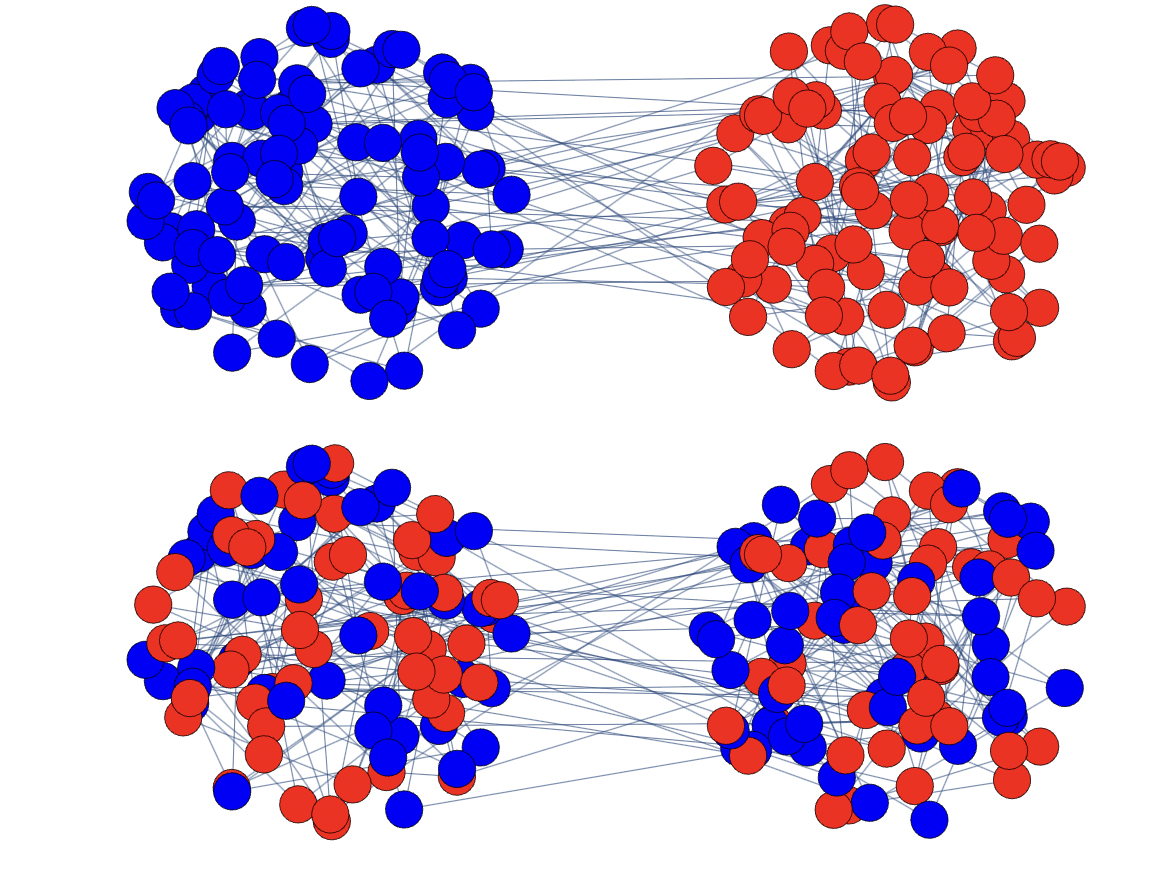
\includegraphics[width=0.8\linewidth]{figure/overfit.png}
          \caption{Partition of a random graph}
        \end{figure}
      \end{column}
  
      \begin{column}{0.60\textwidth}
        \begin{itemize}
          \item The top partition has 38 edges crossing while the bottom one has 39.
          \item For optimzer, the top one is ''optimal" but actually there is no community. 
        \end{itemize}
      \end{column}
    \end{columns}
\end{frame}



\begin{frame}
  \frametitle{Introduction: The community detection from the perspective of physics}

  \begin{itemize}
      \item In computer science, we think \alert{worst-case instances} for evaluating algorithms.
      \item However, the real world networks are rarely worst-case instances.
      \item In physics, we think \alert{typical instances} for evaluating models. (e.g. thermodynamics) \\
      $\Rightarrow$ It is natural to use physical perspective to evaluate the community detection models.
  \end{itemize}
\end{frame}



\begin{frame}
  \frametitle{二段組}

  \begin{columns}
    \begin{column}{0.48\textwidth}
        \begin{itemize}
          \item 文字
          \item 表
        \end{itemize}
    \end{column}

    \begin{column}{0.48\textwidth}
        \begin{figure}
          \centering
          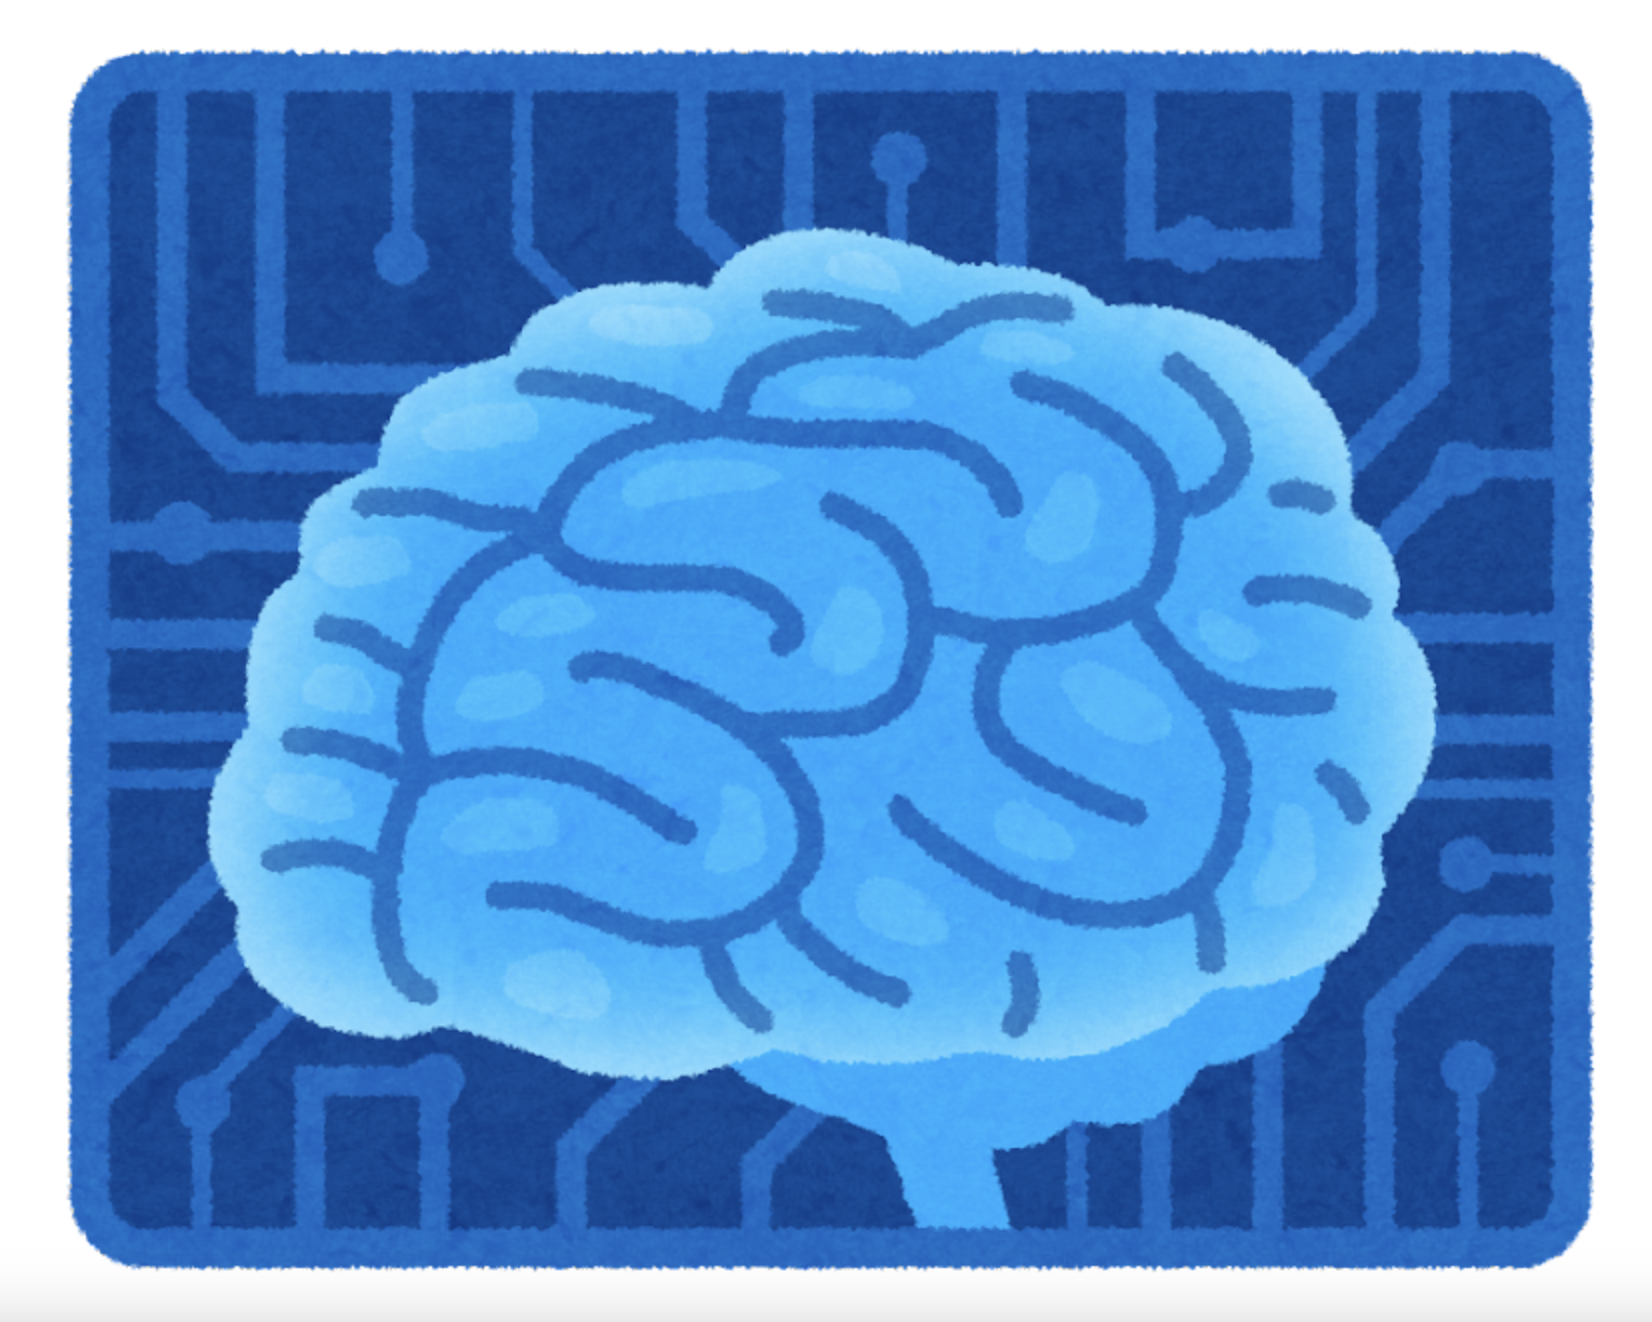
\includegraphics[width=0.8\linewidth]{figure/sample.png}
          \caption{図}
        \end{figure}
    \end{column}
  \end{columns}


\end{frame}


\begin{frame}
  \frametitle{Problem setting}
  \begin{itemize}
    \item Sparse and symmetric stochastic block model (SBM)
    \begin{itemize}
      \item $n$:  $\#$ nodes
      \item $q$:  $\#$ communities
      \item each node $i$ belongs to a community $\sigma_i \in \{1, \dots, q\}$
      \item if $i$ and $j$ belong to the same community, $A_{ij} \sim \text{Bern}(p_{in})$
      \item if $i$ and $j$ belong to different communities, $A_{ij} \sim \text{Bern}(p_{out})$
      \item $p_{in} = c_{in} / n$ and $p_{out} = c_{out} / n$ where $c_{in}$ and $c_{out}$ are constants.
    \end{itemize}
    \item In this model, the expected degree of each vertex is 
    \begin{align}
      c = \frac{n}{q} \times {p_{in}} + \qty(1-\frac{n}{q})\times{p_{out}} = \frac{c_{in} + (q-1) c_{out}}{q}
    \end{align}
    \item Note that Eronds-Renyi model is a special case of SBM where $G(n, p=c/n)$.
\end{itemize}
\end{frame}

\begin{frame}
  \frametitle{Goal}
  There are several types of goal in the community detection problem when $G$ generated from SBM is given.
  \begin{itemize}
    \item \alert{Exact reconstruction}: Finding the planted assignment exactly up to a global permutation.
    \item \alert{Reconstruction (weak recovery)}: Finding the planted assignment whose accuracy is better than random guess ($1/q$).
    \item \alert{Detection}: Hypothesis testing whether $G$ is generated from SBM or Eronds-Renyi model.
  \end{itemize}
  In this talk, we assume $c_{in}$ and $c_{out}$ are known and focus on the reconstruction and detection problems, which are strongly analogous to physics.
\end{frame}

\begin{frame}
  \frametitle{Preparation: Statistical physics and Ising model}
  \begin{itemize}
    \item Statistical physics is a study of macroscopic properties of a system from microscopic properties.
    \item \alert{Ising model}: a simple but fundamental model of magnetism and phase transition.
    \begin{itemize}
      \item There are $n$ atoms on a lattice $G = (V, E)$ and each atom has a spin $\sigma_i \in \{-1, 1\}$.
      \item Neighboring atoms tend to align their spins, so the energy of the system is
      \begin{align*}
        H(\sigma) = - J \sum_{(i, j) \in E}  \delta_{\sigma_i, \sigma_j}.
      \end{align*}
      \item The probability of the system in equilibrium is given by the Boltzmann distribution
      \begin{align*}
        P(\sigma) \propto \exp(- H(\sigma) / T) = \exp( \frac{J}{T} \sum_{(i, j) \in E}  \delta_{\sigma_i, \sigma_j}),
      \end{align*}
      where $T$ is the temperature.
    \end{itemize}
  \end{itemize}
\end{frame}

\begin{frame}
  \frametitle{Preparation: Statistical physics and Ising model}
  There is a \alert{phase transition} in the Ising model, which is a sudden change of the macroscopic properties of the system.
  \begin{figure}
    \centering
    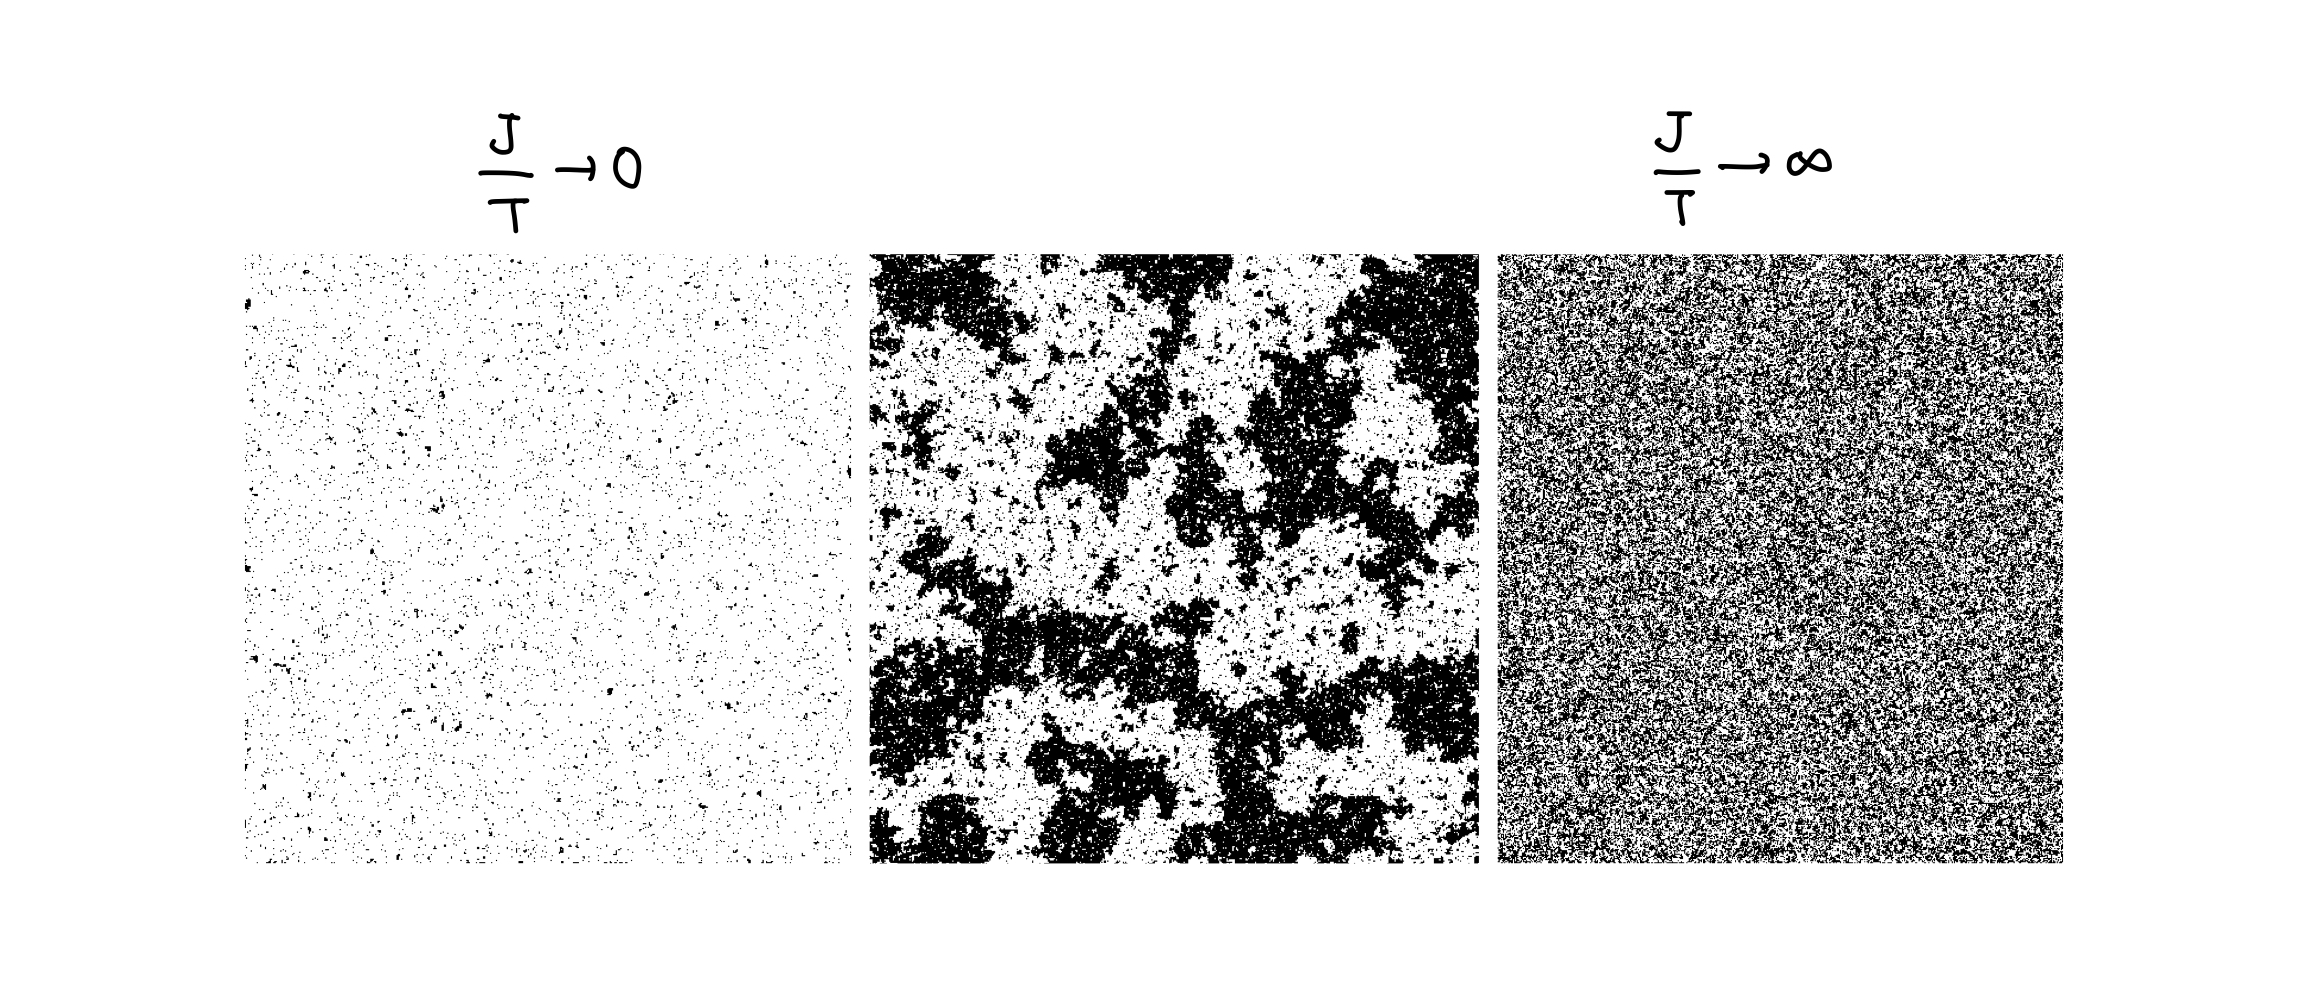
\includegraphics[width=0.6\linewidth]{figure/ising.jpeg}
    \caption{A typical states of the Ising model}
  \end{figure}
  \begin{itemize}
    \item When $J$ is large, the system is in the \alert{ferromagnetic phase} where the spins are aligned.
    \item When $J$ is small, the system is in the \alert{paramagnetic phase} where the spins are randomly distributed.
    \item The change between these phases is sudden: \alert{phase transition}.
  \end{itemize}
  
\end{frame}

\begin{frame}
  \frametitle{Community detection as a statistical physics problem}
  In our model, the probability distribution of $\sigma$ is given by
  \begin{align*}
    & ~~~~ P(\sigma \mid G) \\
    &\propto P(G \mid \sigma) \\
    & = \prod_{(i, j) \in E}  p_{\sigma_i, \sigma_j} \prod_{(i, j) \notin E} (1 - p_{\sigma_i, \sigma_j}) \\
    & = \prod_{(i,j) \in E} \qty(\frac{p_{in}}{p_{out}})^{\delta_{\sigma_i, \sigma_j}} \prod_{(i, j) \notin E}   \qty(1 - \frac{p_{in}}{p_{out}})^{1 - \delta_{\sigma_i, \sigma_j}} \\
    & = \exp(\log(\frac{p_{in}}{p_{out}}) \sum_{(i, j) \in E}  \delta_{\sigma_i, \sigma_j} + \log(1 - \frac{p_{in}}{p_{out}}) \sum_{(i, j) \notin E}  (1 - \delta_{\sigma_i, \sigma_j})) \\
    & \sim \exp(\log(\frac{p_{in}}{p_{out}}) \sum_{(i, j) \in E}  \delta_{\sigma_i, \sigma_j} )
  \end{align*}
\end{frame}

\begin{frame}
  \frametitle{Community detection as a statistical physics problem}
  \begin{itemize}
    \item In conclusion, the community detection problem is equivalent to the Ising model with $J/T = \log(\frac{p_{in}}{p_{out}})$ in a simple approximation.
    \item From an analogy of the phase transition in the Ising model, we can expect the phase transition in the community detection problem.
  \end{itemize}
\end{frame}





\end{document}




